% \chapter{WFP mVAM Data: a Case Study}

Food insecurity, defined as the inability of households to gain access to sufficient, safe and nutritious food that meets dietary needs and food preferences for an active and healthy life, is a pervasive global issue. Between 2020 and 2022, the COVID-19 pandemic exacerbated global food insecurity by disrupting markets, reducing household incomes, and straining public health systems~\cite{Mueller, Pereira}. Pandemic impacts were particularly severe in regions already experiencing humanitarian crises, with the disintegration of preexisting food systems resulting in increased malnutrition and susceptibility to disease~\cite{Pritchard}. An additional challenge in responding to both chronic and acute food insecurity during the COVID-19 pandemic was the inability to collect data to monitor beneficiary populations using traditional methods due to travel restrictions and quarantine orders. High-frequency phone surveys were rapidly adopted as an alternative in many countries, but the inconsistent performance of these tools highlighted the need for careful consideration in the design and implementation of remote data collection systems~\cite{Gourlay,Ratrikaningtyas}. The mobile Vulnerability Analysis and Mapping (mVAM) system developed by the World Food Programme (WFP) between 2013 and 2015~\cite{Mock_PE, Morrow_PE} was one of the few remote data collection tools already in place prior to the onset of the COVID-19 pandemic, and high-frequency data from mVAM surveys in nearly 30 countries became a critical resource for monitoring food security in populations at the regional and national level~\cite{WFP_mVAM}.

Daily participants in national phone-based surveys conducted to collect mVAM data are determined by random sampling from a large population of households, stratified at the regional level, with a different random sample taken each day to obtain a target number of responses. The standard use of high-frequency data collected by mVAM is to provide real-time tracking of household consumption levels and the use of coping strategies to mitigate food shortages, with results rapidly aggregated and smoothed using a thirty-day moving window to support WFP's HungerMap\textsuperscript{LIVE} application (\url{https://hungermap.wfp.org/}). In addition to collecting data on consumption patterns, access to assistance, and household coping strategies, mVAM surveys also collect various demographic factors. Depending on the setting, respondents may be asked to report the size of their households, residency status, the sex of the head of household, income sources, and education. As a result, mVAM data enable not only the estimation of long-term trends, but also offer the potential to assess the impact of household-level covariates on reported food insecurity. 

\subsection*{Food security indicators}\label{FS_defs}
Standard analyses of mVAM survey data focus on two key food security indicators, the Food Consumption Score (FCS) and the Reducing Coping Strategies Index (rCSI). Initially developed by WFP in 1996, the FCS is a summary statistic intended to measure dietary adequacy from both a nutritional and caloric standpoint~\cite{WFP_FCS_2024}. Respondents are asked to state the number of days in the previous week that members of their household consumed foods from a standard list of groups, based on the assumption that meals in the household are communal. The FCS is computed by taking a weighted average of the days of consumption of eight major food groups (Starches, Vegetables, Fruits, Pulses, Dairy, Animal Proteins, Fats, and Sugar), according to the following formula: $\mbox{FCS} = (\mbox{Starches}\times 2)+ (\mbox{Pulses}\times 3)+ \mbox{Vegetables} + \mbox{Fruit} + (\mbox{Meat}\times 4)+ (\mbox{Dairy}\times 4)+ (\mbox{Fats}\times .5)+ (\mbox{Sugar} \times.5).$ The weights sum to 16, and the maximum attainable score is 112. In its reporting, WFP defines FCS thresholds to classify households into three consumption levels. In Honduras, households scoring at or below 28 are considered to have a poor level of consumption, as a score this low would be associated with consuming little other than starches, fats, and sugar on a daily basis. Households scoring between 29 and 42 have inadequate or borderline levels of consumption, while households scoring 43 or above are considered to have adequate consumption~\cite{WFP_FCS_2024}.

The rCSI is a food security indicator developed by the WFP and CARE to measure the frequency and severity of food-related coping strategies used by households when faced with insufficient food or resources to purchase food~\cite{rCSI}. It is based on a seven-day recall period covering five standard behaviors: (1) relying on less preferred or less expensive foods; (2) borrowing food or relying on help from friends or relatives; (3) limiting portion sizes at mealtimes; (4) restricting consumption by adults so that children can eat; and (5) reducing the number of meals eaten per day. Each behaviour is assigned a severity weight (1, 2, 1, 3, and 1, respectively), and the household’s rCSI is calculated by multiplying the reported frequency (days) of each behaviour by its weight and summing across all five strategies. Higher scores indicate greater reliance on coping strategies and, therefore, poorer food security. Although there are no universally implemented thresholds for rCSI scores, the Integrated Food Security Phase Classification (IPC) considers a score of 19 or above to represent moderate food insecurity~\cite{cfi}.


\subsection{mVAM in Honduras}

The dataset considered for our case study comprises surveys collected in Honduras between April 2020 and September 2023, during which time 54,208 responses were recorded following informed consent protocols established by the World Food Programme. An average of roughly 45 households per day were randomly selected, with varying numbers of responses recorded at the department (regional) level. Demographic information for each household included geographic location at the district level (including whether the location was rural, a small city, or a large city), the gender and age of the respondent, the sex and education level of the head of household, the size of the household, and the household's primary and secondary income sources. Questions about the household's ability to access medical care and educational services were also included due to COVID-19 restrictions. Questions about food consumption and coping strategies needed to construct the FCS and rCSI indicators were included, and respondents were also asked to report whether they had received any type of assistance from the government or NGOs. These data were deidentified by WFP analysts and shared with our research team via an agreement with the US Agency for International Development in August 2023. 

In addition to experiencing economic disruptions due to COVID-19, Honduras was hit by two major storms, Hurricanes Eta and Iota, in November 2020. Our analysis focuses on 5 departments that were significantly impacted by major flooding and landslides: Col{\'o}n, Cort{\'e}s, Gracias a Dios, Santa B{\'a}rbara, and Yoro~\cite{CERF}. Based on regional aggregates, nearly 20\% of the households surveyed in these departments had inadequate consumption through fall 2021 while over 40\% of the households engaged in crisis or emergency-level food coping during the same time period, with notable improvements in both indicators observed in 2022 (Figure~\ref{fig:single_sim_inf}). However, economic, political and environmental shocks continued to impact the country, with an uptick in food security observed in early 2023~\cite{HondurasReport2023}. 

\begin{figure}[htbp]
    \centering
    \begin{subfigure}{\textwidth}
        \centering
        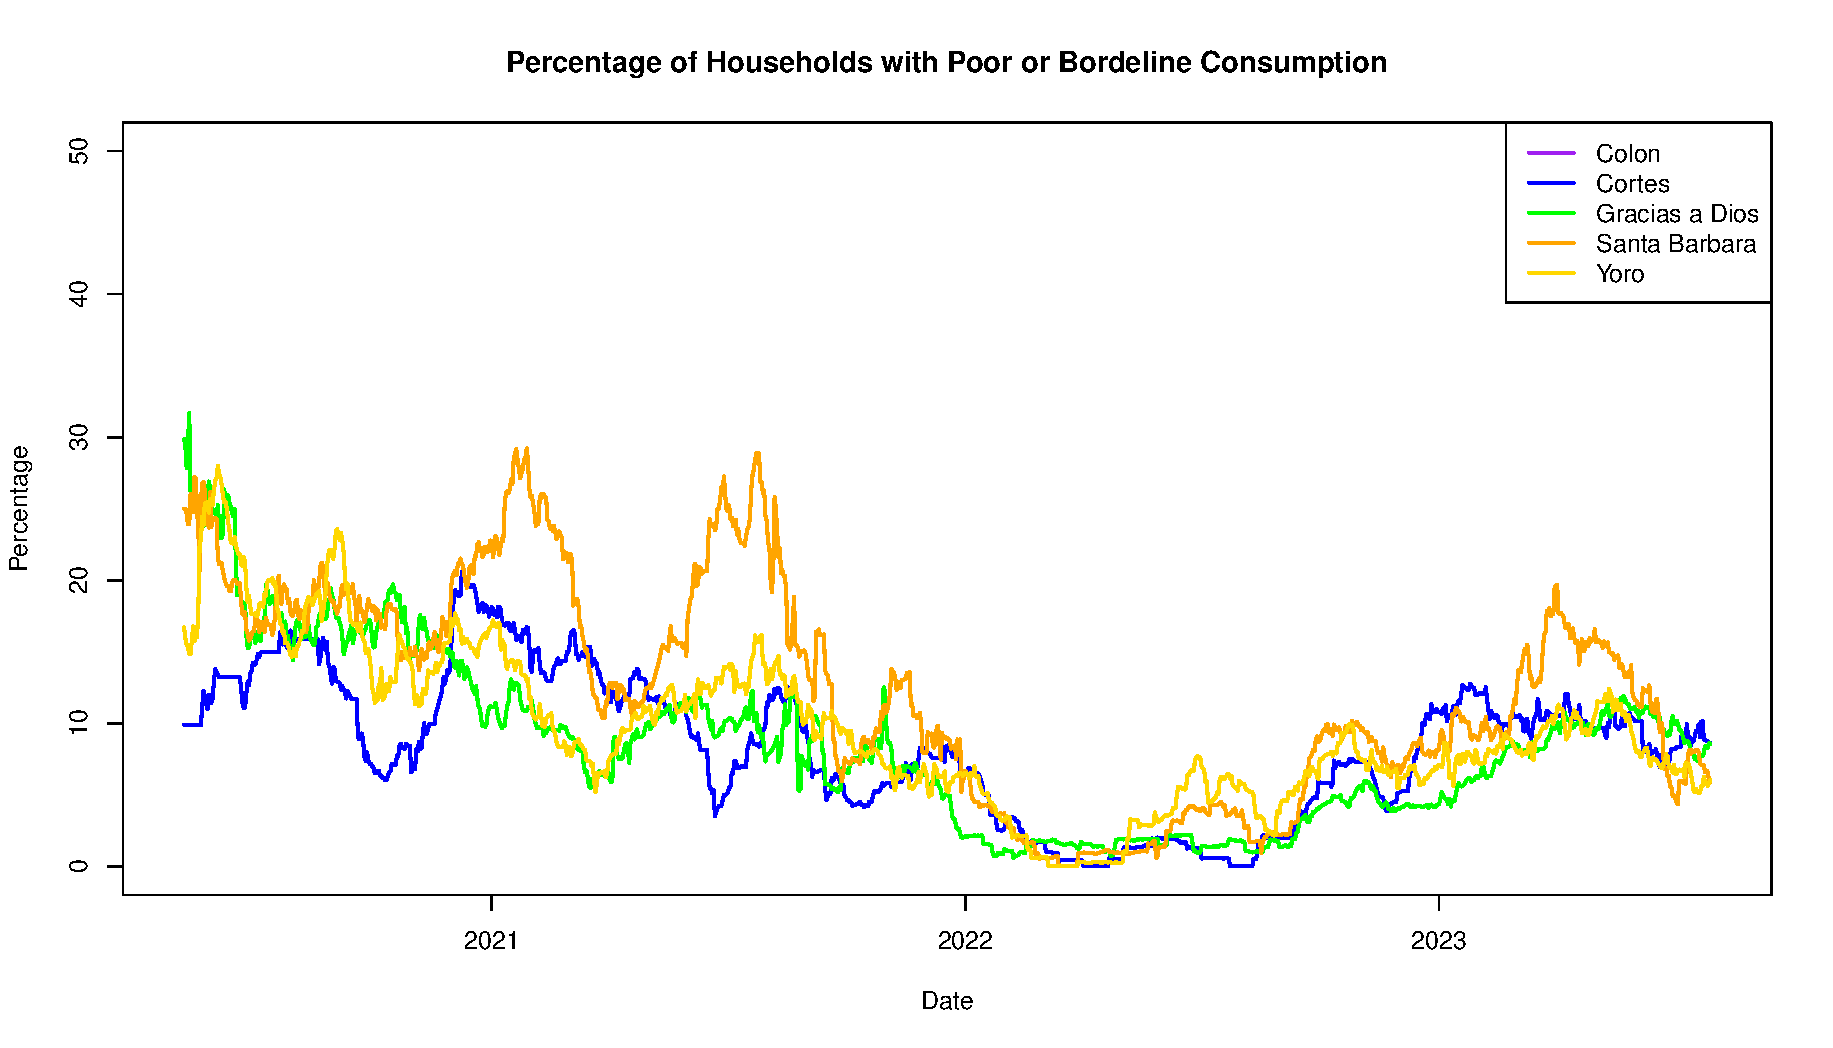
\includegraphics[width=\linewidth]{images/WFP_FCS_Summary.pdf}
    \end{subfigure}
\vspace{.2in}
    \begin{subfigure}{\textwidth}
        \centering
        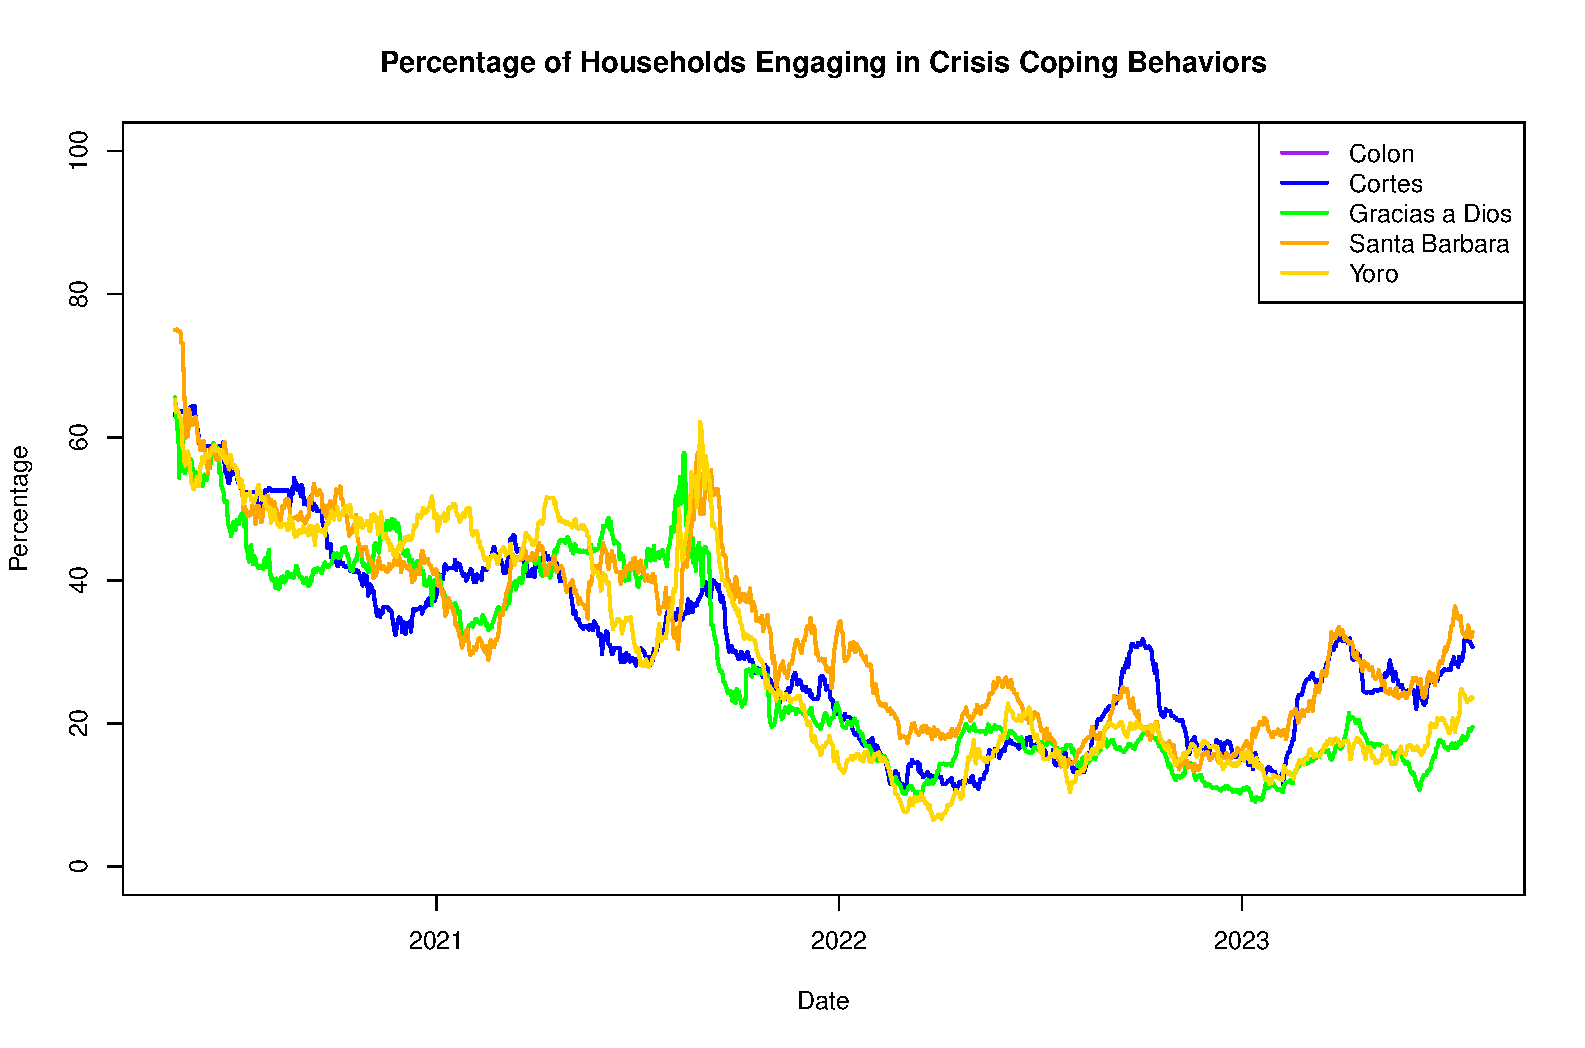
\includegraphics[width=\linewidth]{images//output/WFP_rCSI_Summary.pdf}
    \end{subfigure}
    \caption{WFP estimates from aggregated FCS scores (top) and rCSI scores (bottom) in five hurricane-impacted departments}
    \label{fig:single_sim_inf}
\end{figure}

% \begin{figure}
%     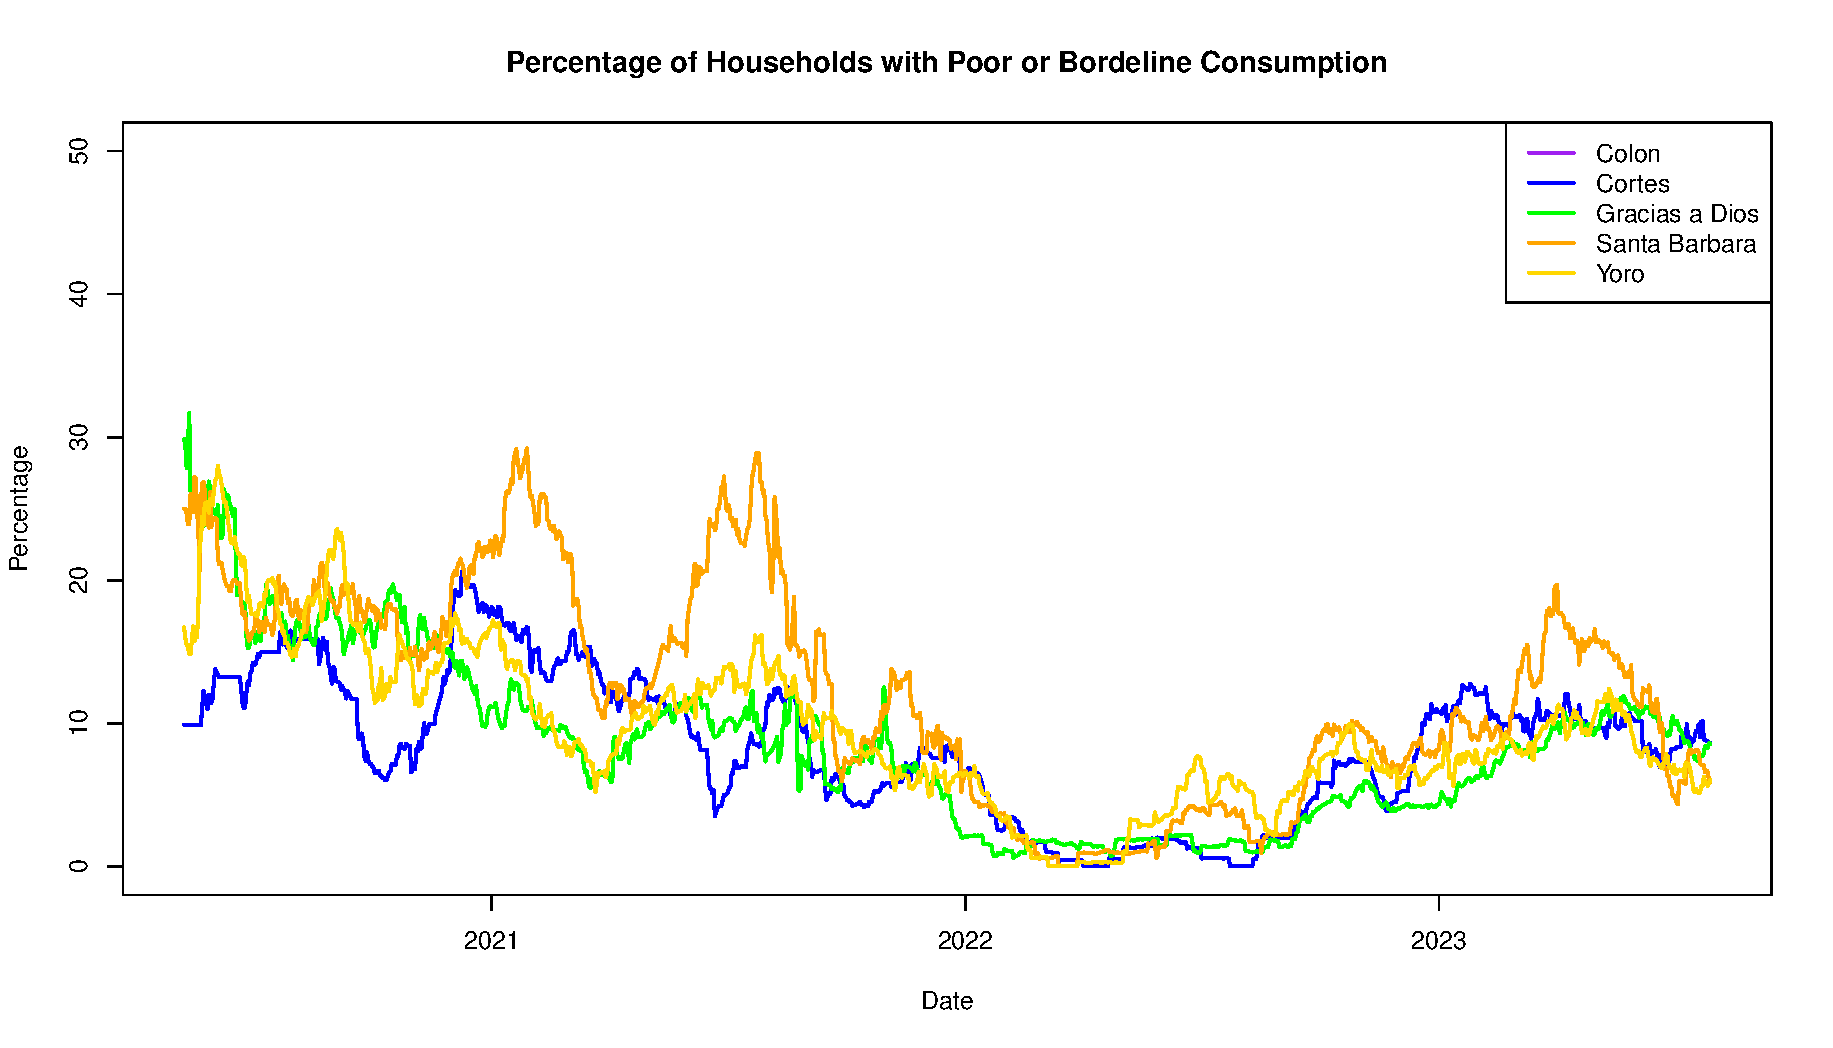
\includegraphics[width=1\linewidth]{images/WFP_FCS_Summary.pdf}
%     \caption{WFP estimates from aggregated FCS scores}
%     \label{fig:FCS.agg}
% \end{figure}
% \begin{figure}[H]
%     \centering
%     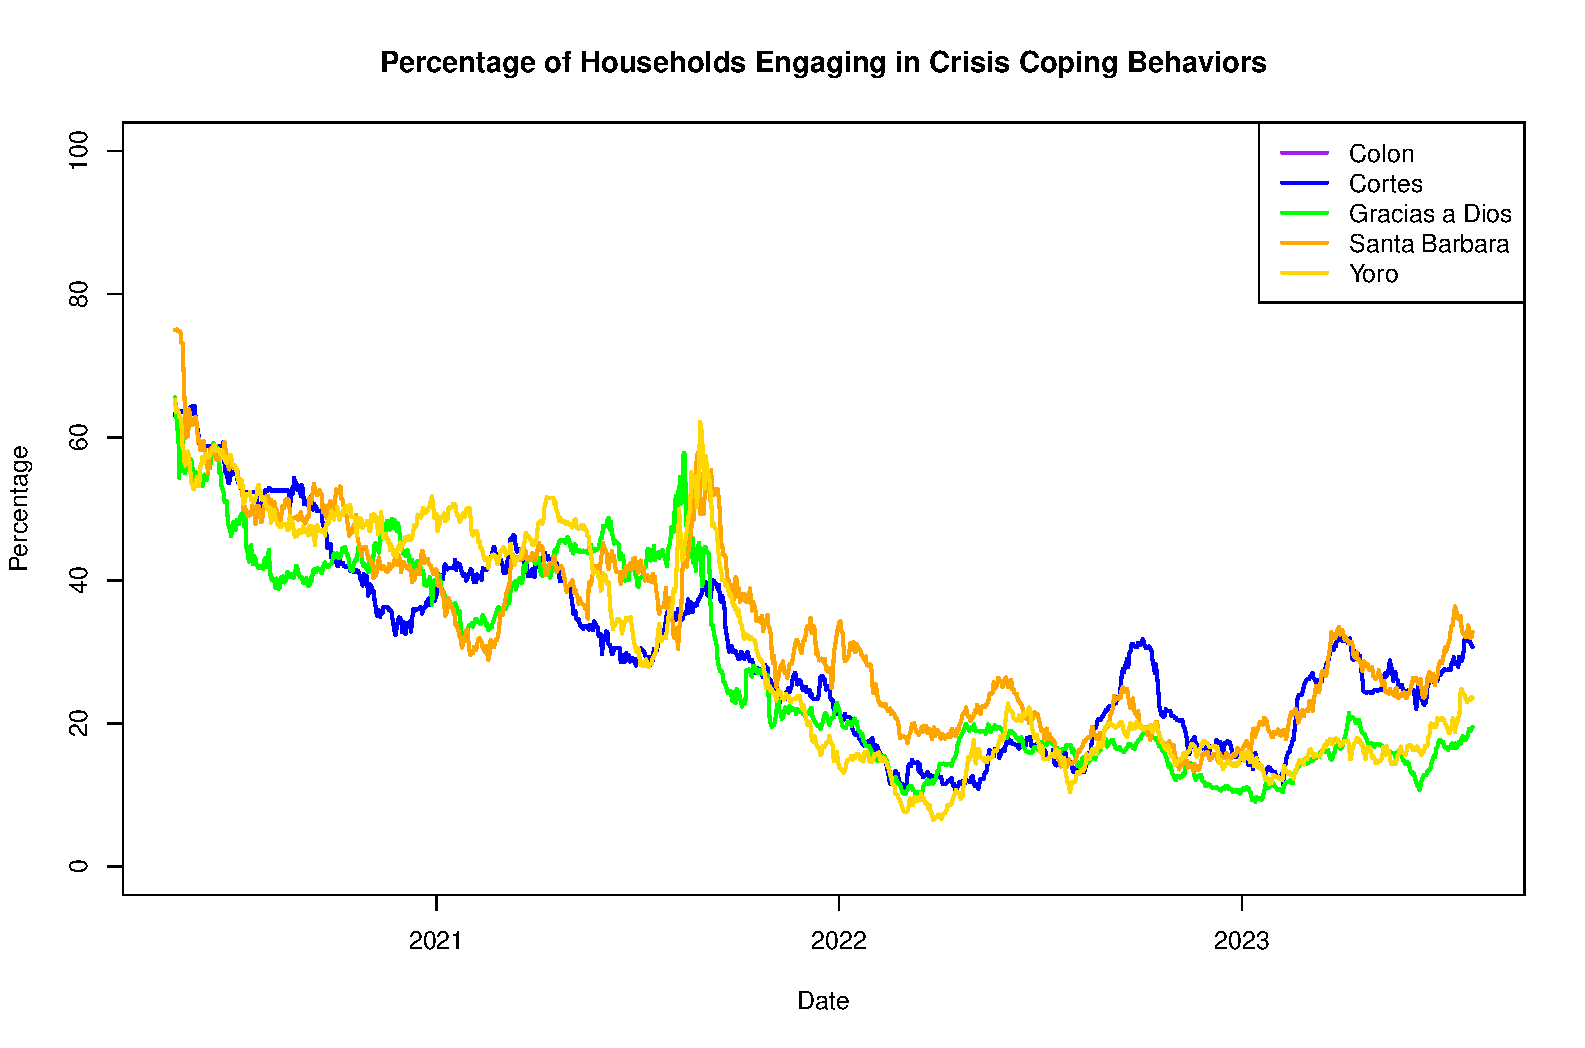
\includegraphics[width=1\linewidth]{images//output/WFP_rCSI_Summary.pdf}
%     \caption{WFP estimates from aggregated rCSI scores}
%     \label{fig:rCSI.agg}
% \end{figure}

\section{Modeling Results}    
While the summaries produced by WFP provide insights into aggregate trends, at the household level the average standard deviation in FCS scores was 15 points, indicating extremely high variability. For this reason, it is important to understand the key factors determining individual consumption levels. We began by fitting a standard regression model, with results indicating that variability in FCS scores was significantly associated with location (both department and population density), education level, household size, head of household sex, primary occupation, and receipt of assistance. We also included a time variable with both linear and squared terms to fit an overall quadratic trend.

Residuals from the fitted model, which explained 13\% of the variability in the data, were approximately normally distributed, but clearly displayed a high degree of temporal correlation as shown in Figure~\ref{fig:FCS_orig_res}. After running the REMARCS algorithm, model residuals were no longer correlated (see Figure~\ref{fig:FCS_remarcs_res}). The ARMA(1,1) model estimated by REMARCS had parameters $\hat{\phi}=0.98, \hat{\theta}=-0.85$, indicating strong autocorrelation with the potential for abrupt directional shifts. The REMARCS model also had a smaller residual standard error, decreasing from 15.51 for the OLS model to 15.07. 

\begin{figure}
    \centering
    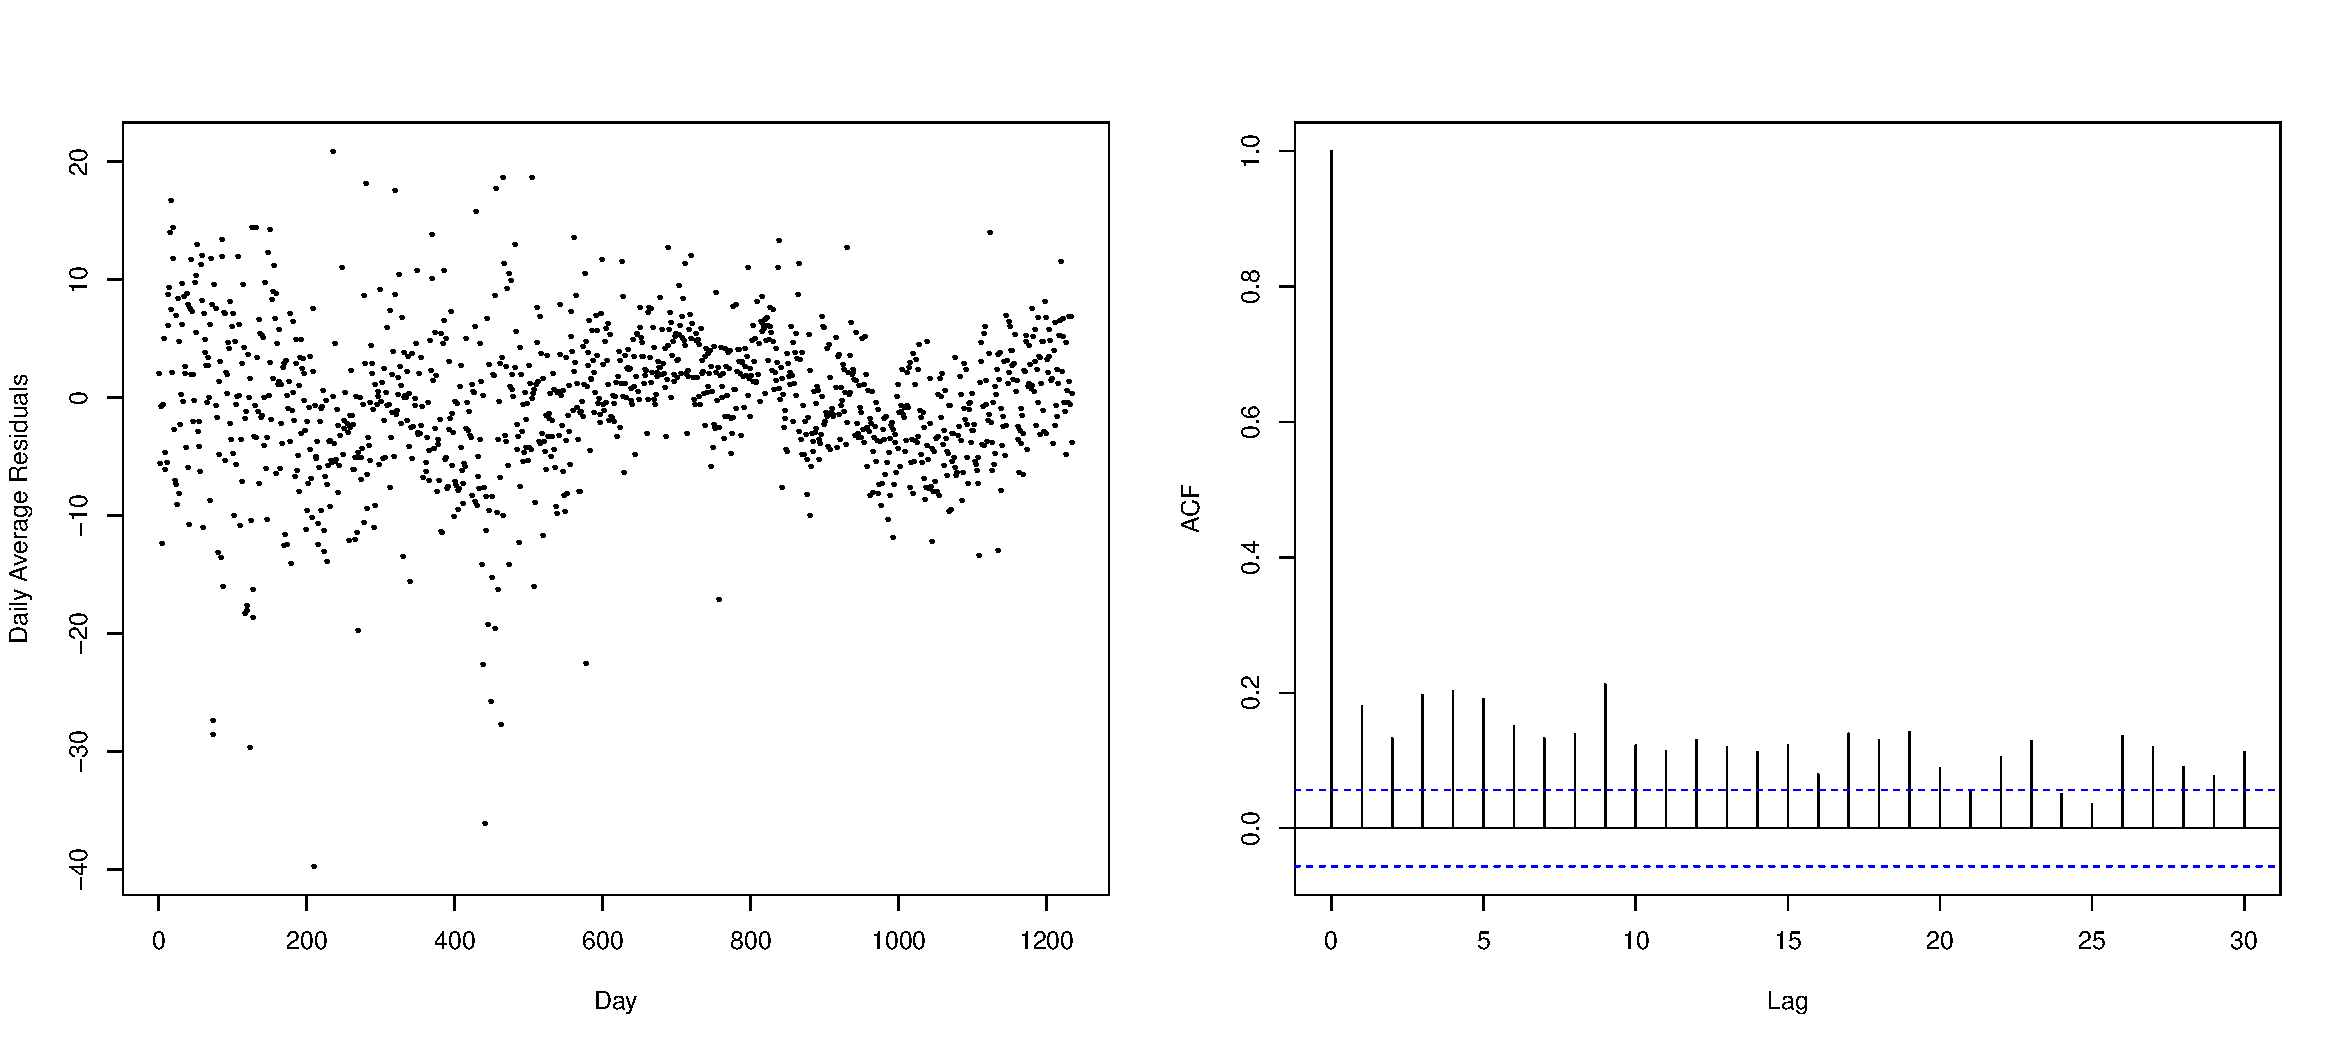
\includegraphics[width=1\linewidth]{images/FCSmod_orig_dailyres.pdf}
    \caption{Left: Average daily residuals from the fitted regression model for FCS. Right: Autocovariance plot for average daily residuals}
    \label{fig:FCS_orig_res}
\end{figure}

\begin{figure}
    \centering
    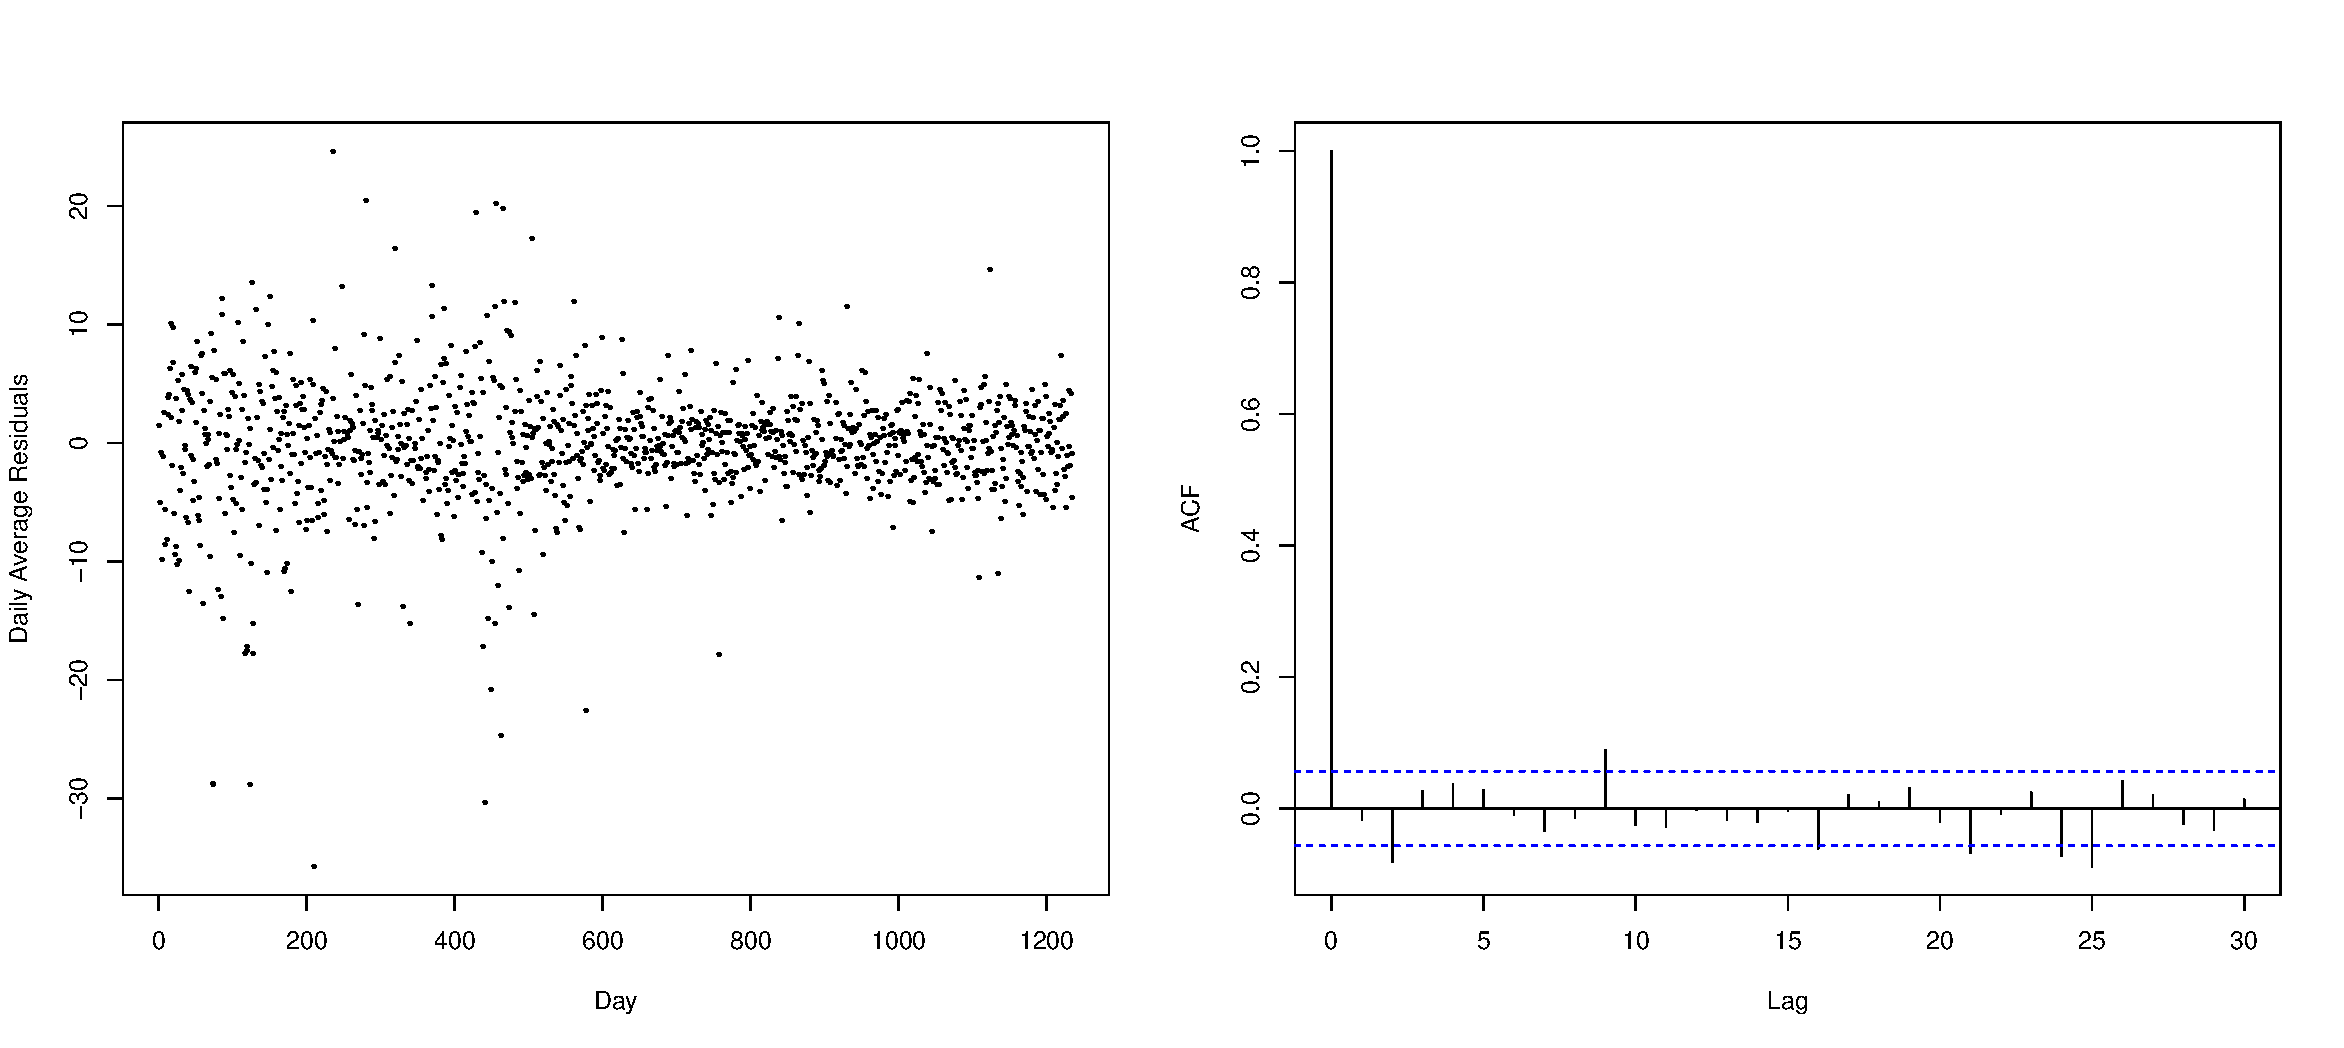
\includegraphics[width=1\linewidth]{FCSmod_rcs_dailyres.pdf}
    \caption{Left: Average daily residuals from the fitted REMARCS model for FCS. Right: Autocovariance plot for average daily residuals}
    \label{fig:FCS_remarcs_res}
\end{figure}

 While the REMARCS model retained the same covariates as statistically significant as for the OLS model, there were some differences in model coefficients and their associated standard errors (see Table~\ref{tab:FCS_tab}). In both cases, the fitted models indicated significant differences in average consumption levels across the five departments. Households in small cities had higher average consumption than rural households (set as the baseline level and included in the intercept term), which in turn had higher average consumption than residents of large cities. Education was highly significant and followed an increasing trend, with the highest consumption levels estimated for households with education beyond the primary level (illiteracy was the baseline level). Households headed by both sexes fared better than either male (baseline) or female-headed households, while consumption levels were inversely associated with household size. Households receiving assistance, lacking a regular income source, or relying on charity/NGO support had lower average consumption than those with regular formal employment (informal daily labor was the baseline level). Notable changes in parameters associated with the REMARCS model were increases in the magnitudes of parameters associated with department, population density, and assistance.   

\begin{sidewaystable}
    \small
    \centering
    \begin{tabular}{lrrrr}
        Covariate	&	OLS Estimate	&	OLS Std. Error	&	REMARCS Estimate	&	REMARCS Std. Error	\\
Intercept	&	55.55892	&	0.69983	&	56.00315	&	1.99251	\\
Department: Cort{\'e}s	&	1.49768	&	0.38220	&	1.48454	&	0.38490	\\
Department: Gracias a Dios	&	-1.29787	&	0.44037	&	-1.37484	&	0.44108	\\
Department: Santa B{\'a}rbara	&	-2.00598	&	0.39614	&	-2.06755	&	0.39374	\\
Department: Yoro	&	-2.04978	&	0.38499	&	-2.08285	&	0.38261	\\
Day	&	0.01799	&	0.00150	&	0.01627	&	0.00714	\\
$Day^2$	&	-0.00002	&	0.00000	&	-0.00002	&	0.00001	\\
Pop Density: Large City	&	-1.11153	&	0.35924	&	-1.57302	&	0.35999	\\
Pop Density: Small City	&	1.24400	&	0.30561	&	0.90564	&	0.30517	\\
Education: Primary	&	4.63793	&	0.48226	&	4.69604	&	0.48044	\\
Education: Seconday	&	8.03498	&	0.49925	&	7.93902	&	0.49882	\\
Education: University	&	11.15058	&	0.62775	&	11.10039	&	0.62533	\\
Education: VocationalTraining	&	9.18409	&	0.65478	&	9.32931	&	0.65285	\\
Household Size	&	-0.26260	&	0.05162	&	-0.26451	&	0.05150	\\
Head of Household Sex: Both	&	0.92264	&	0.29633	&	0.95552	&	0.29590	\\
Head of Household Sex: Female	&	-0.56173	&	0.35912	&	-0.34456	&	0.35684	\\
Assistance Received	&	-0.88059	&	0.28658	&	-1.29160	&	0.28714	\\
Primary Income: Business/SelfEmployed	&	4.77979	&	0.49561	&	4.82818	&	0.49346	\\
Primary Income: Housecleaning/CareWork	&	-1.69638	&	0.69574	&	-1.94788	&	0.69167	\\
Primary Income: GovAssistance/Pension	&	-0.29584	&	1.24207	&	-0.63630	&	1.23308	\\
Primary Income: Informal Trade	&	0.33543	&	0.48890	&	0.43442	&	0.48585	\\
Primary Income: None	&	-8.43743	&	0.56936	&	-8.34208	&	0.56743	\\
Primary Income: Remittances/Family/Friends	&	2.95203	&	1.03774	&	2.61032	&	1.03059	\\
Primary Income: Salaried Work	&	3.95280	&	0.33419	&	3.91366	&	0.33364	\\
Primary Income: Charity/NGO/WFP	&	-13.54970	&	7.76009	&	-13.76163	&	7.71296	\\
$\phi$ (AR parameter)	&	NA	&	NA	&	0.97660	&	0.00964	\\
$\theta$ (MA parameter)	&	NA	&	NA	&	-0.85316	&	0.02823	\\
    \end{tabular}
    \caption{Caption: Parameter Estimates and Standard Errors from OLS and REMARCS Models for FCS}
    \label{tab:FCS_tab}
\end{sidewaystable}


To illustrate the differences between the two models, we compare predictions for a ``typical'' respondent in C{\'o}lon, characterized as a rural household with five individuals, headed by a male with a primary education and informal daily labor as the primary income source. The OLS model predicted an FCS score gradually increasing from 59 in spring 2020 to 63 in late 2022 before declining to 53 in 2023. The REMARCS model, on the other hand, predicted a much more volatile trajectory, with large drops in late 2020 and late 2022 that likely reflected a response to environmental and economic shocks (see Figure~\ref{fig:FCS_pred_comp}).

\begin{figure}[H]
    \centering
    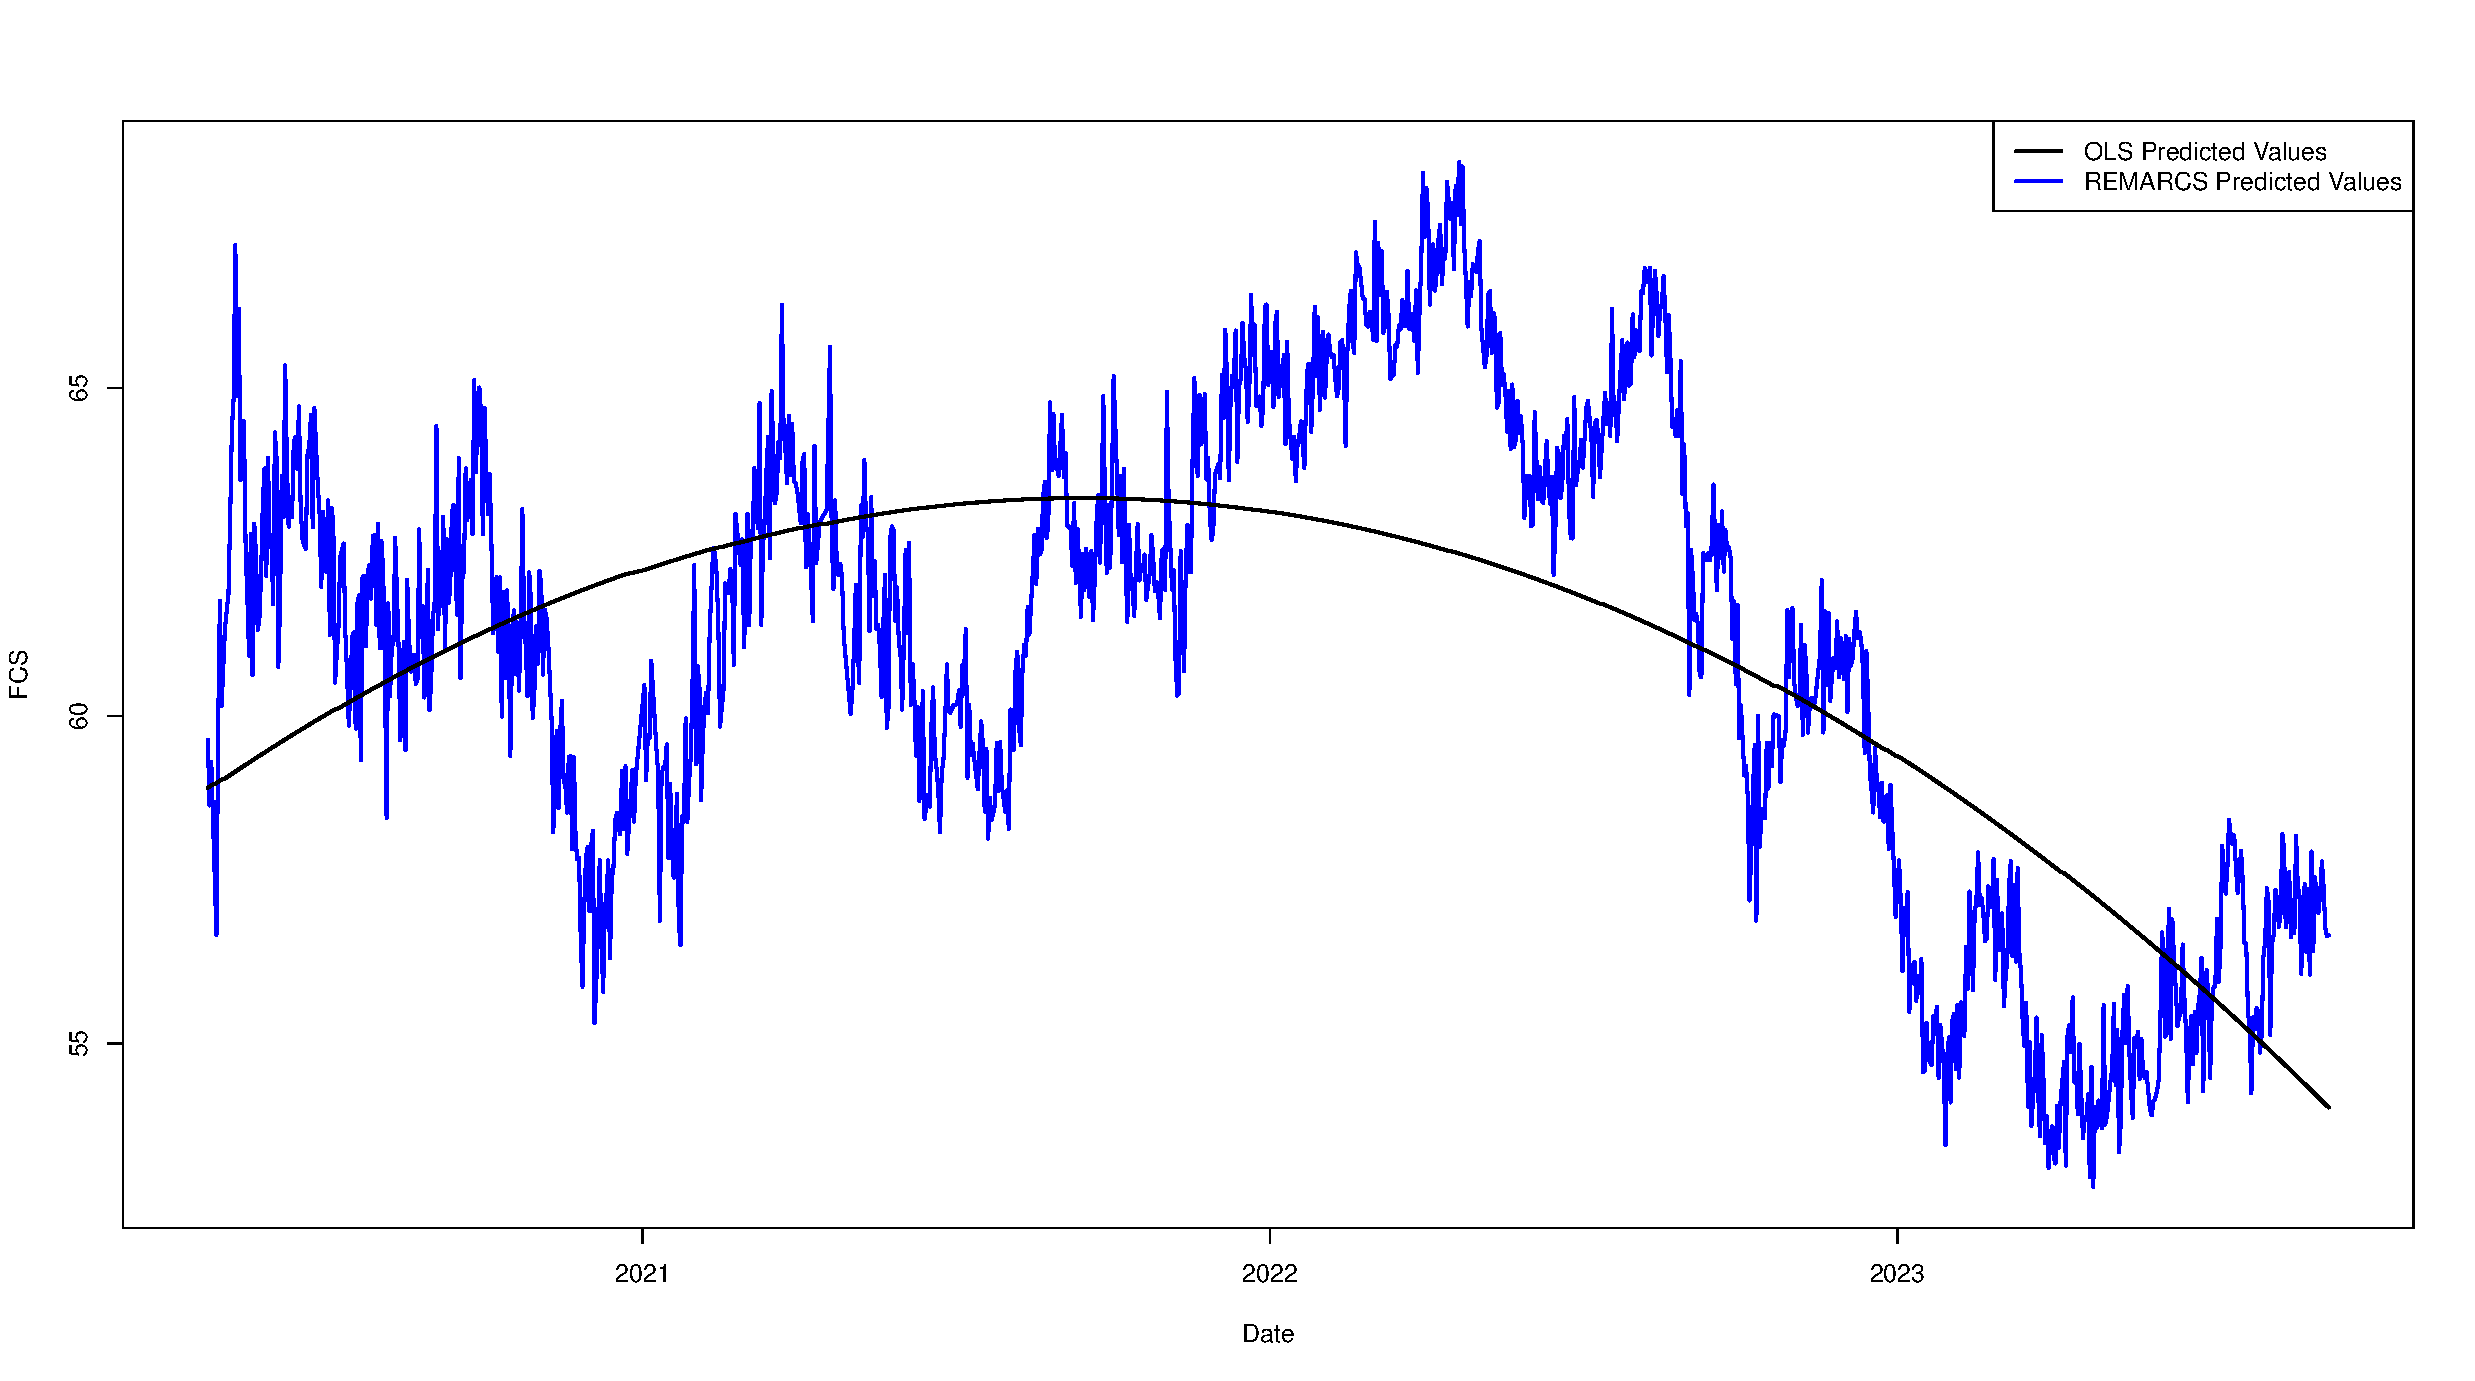
\includegraphics[width=1\linewidth]{FCSmod_predictions.pdf}
    \caption{Predicted FCS values for a typical household from OLS and REMARCS models}
    \label{fig:FCS_pred_comp}
\end{figure}

For the rCSI, models were fit after taking the square root of the observations to correct for skewness. The OLS model explained 23\% of the variability in $\sqrt{rCSI}$ scores, but once again, residuals indicated significant autocorrelation. This temporal dependence was corrected through the REMARCS model fit (Figures \ref{fig:rCSI_orig_res} and \ref{fig:rCSI_rcs_res}). The estimated ARMA(1,1) model was similar to that for FCS, with $\hat{\phi}$=0.96 and $\hat{\theta}$=-0.83, and the residual standard error decreased from 1.25 to 1.23.   

\begin{figure}[H]
    \centering
    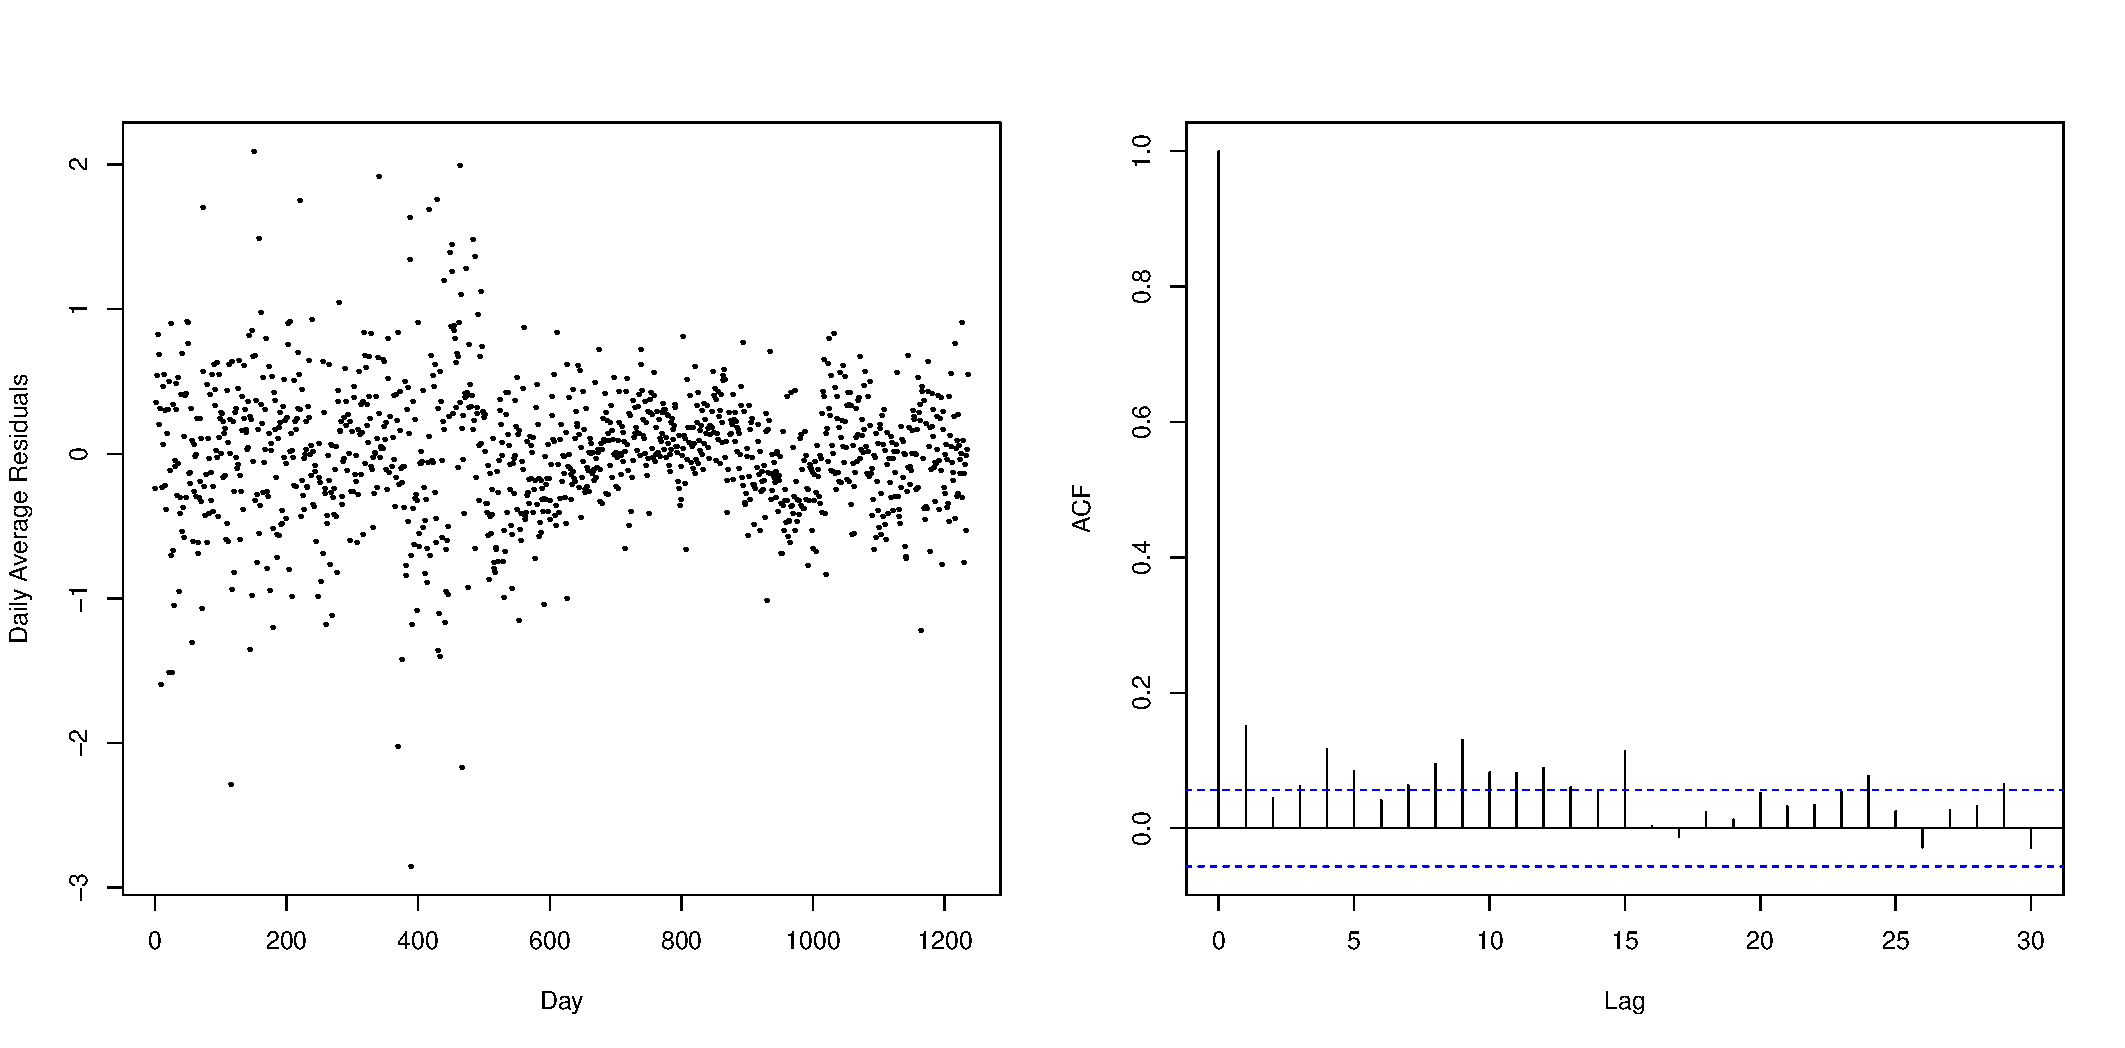
\includegraphics[width=1\linewidth]{images/rCSImod_orig_dailyres.pdf}
    \caption{Left: Average daily residuals from the fitted regression model for $\sqrt{rCSI}$. Right: Autocovariance plot for average daily residuals}
    \label{fig:rCSI_orig_res}
\end{figure}

\begin{figure}[H]
    \centering
    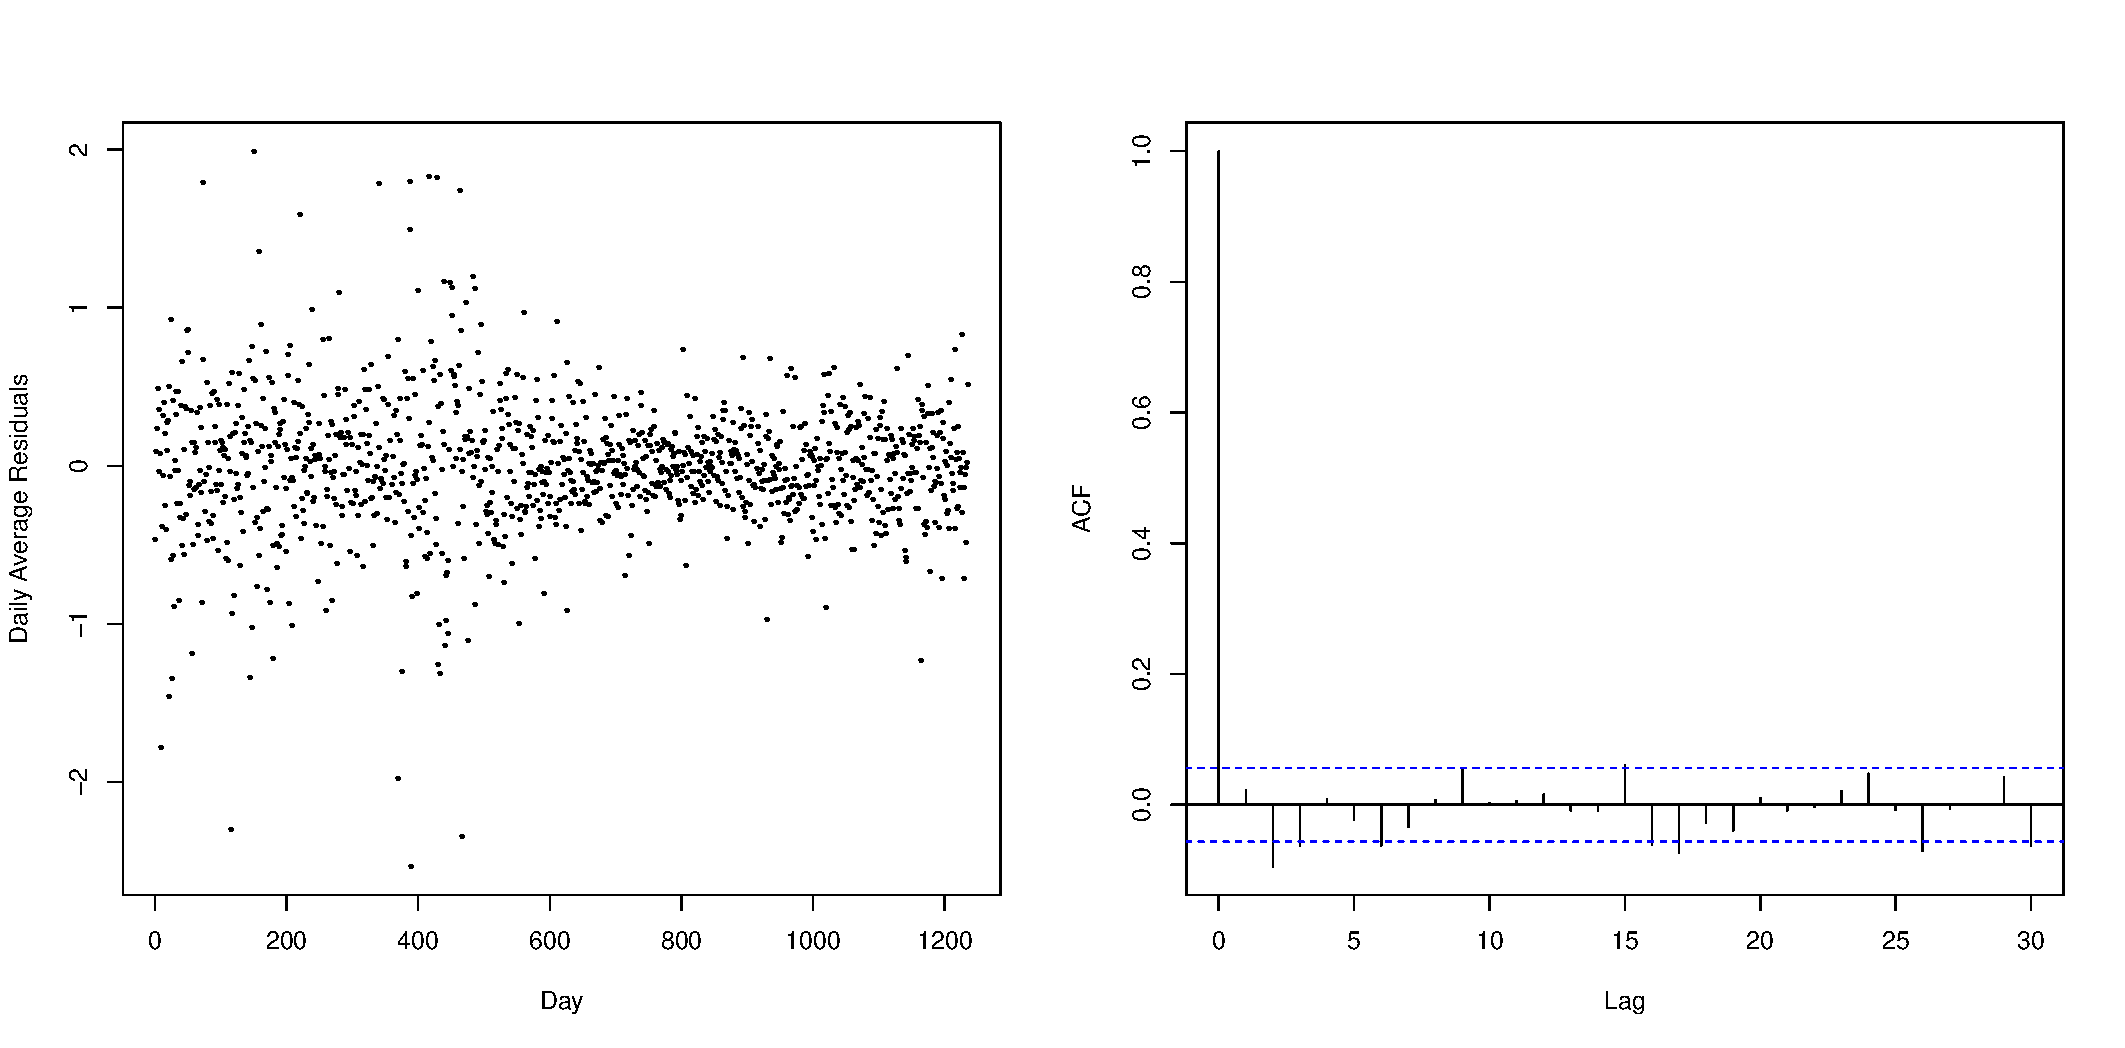
\includegraphics[width=1\linewidth]{images/rCSImod_rcs_dailyres.pdf}
    \caption{Left: Average daily residuals from the fitted REMARCS model for $\sqrt{rCSI}$. Right: Autocovariance plot for average daily residuals}
    \label{fig:rCSI_rcs_res}
\end{figure}

Model coefficients differed in some important ways than for the FCS model, with lower average coping levels estimated for urban residents (in both small and large cites) than for rural households (Table~\ref{tab:rCSI_tab}). Specifically, female-headed households were predicted to have significantly higher $\sqrt{rCSI}$ scores than male-headed households, although households headed by both sexes had the lowest average predicted scores. While coefficients associated with educational levels followed the same trends as for the FCS, significantly higher levels of food coping were predicted for households whose primary income source was informal trade or housekeeping/care work. Additionally, these models included an indicator for the sex of the respondent, which reflects the phenomenon that women are more likely to report higher levels of food insecurity than men~\cite{Matheson_McIntyre_2014}.  

\begin{sidewaystable}
    \small
    \centering
    \begin{tabular}{lrrrr}
    Covariate	&	OLS Estimate	&	OLS Std. Error	&	REMARCS Estimate	&	REMARCS Std. Error	\\
Intercept	&	4.462830	&	0.056831	&	4.52E+00	&	1.03E-01	\\
Department: Cort{\'e}s	&	0.158862	&	0.030776	&	1.52E-01	&	3.11E-02	\\
Department: Gracias a Dios	&	0.171668	&	0.035461	&	1.69E-01	&	3.56E-02	\\
Department: Santa B{\'a}rbara	&	-0.008780	&	0.031886	&	-1.25E-02	&	3.18E-02	\\
Department: Yoro	&	0.034962	&	0.030993	&	3.59E-02	&	3.09E-02	\\
Day	&	-0.002090	&	0.000121	&	-2.20E-03	&	3.47E-04	\\
$Day^2$	&	0.000001	&	0.000000	&	1.40E-06	&	2.77E-07	\\
Pop Density: Large City	&	-0.531342	&	0.029015	&	-5.38E-01	&	2.92E-02	\\
Pop Density: Small City	&	-0.186378	&	0.024603	&	-2.00E-01	&	2.47E-02	\\
Education: Primary	&	-0.297135	&	0.038856	&	-2.90E-01	&	3.88E-02	\\
Education: Seconday	&	-0.687499	&	0.040244	&	-6.90E-01	&	4.03E-02	\\
Education: University	&	-0.957933	&	0.050564	&	-9.65E-01	&	5.06E-02	\\
Education: VocationalTraining	&	-0.995288	&	0.052762	&	-9.89E-01	&	5.28E-02	\\
Household Size	&	0.078719	&	0.004156	&	7.72E-02	&	4.17E-03	\\
Head of Household Sex: Both	&	-0.271312	&	0.023904	&	-2.84E-01	&	2.40E-02	\\
Head of Household Sex: Female	&	0.176365	&	0.030291	&	1.72E-01	&	3.02E-02	\\
Respondent Sex: Female	&	0.103970	&	0.021713	&	1.10E-01	&	2.17E-02	\\
Assistance Received	&	0.096715	&	0.023070	&	8.76E-02	&	2.32E-02	\\
Primary Income: Business/SelfEmployed	&	-0.604215	&	0.039922	&	-5.97E-01	&	3.99E-02	\\
Primary Income: Housecleaning/CareWork	&	0.295960	&	0.056121	&	2.89E-01	&	5.60E-02	\\
Primary Income: GovAssistance/Pension	&	-0.276054	&	0.099955	&	-2.80E-01	&	9.97E-02	\\
Primary Income: Informal Trade	&	0.169133	&	0.039364	&	1.68E-01	&	3.93E-02	\\
Primary Income: None	&	-0.133396	&	0.045835	&	-1.16E-01	&	4.58E-02	\\
Primary Income: Remittances/Family/Friends	&	-0.118630	&	0.083500	&	-1.31E-01	&	8.33E-02	\\
Primary Income: Salaried Work	&	-0.364533	&	0.026913	&	-3.57E-01	&	2.70E-02	\\
Primary Income: Charity/NGO/WFP	&	0.058769	&	0.624449	&	1.81E-02	&	6.23E-01	\\
$\phi$ (AR parameter)	&	NA	&	NA	&	0.955443	&	0.018940	\\
$\theta$ (MA parameter)	&	NA	&	NA	&	-0.834486	&	0.039169	\\
\end{tabular}
    \caption{Caption: Parameter Estimates and Standard Errors from OLS and REMARCS Models for $\sqrt{rCSI}$}
    \label{tab:rCSI_tab}
\end{sidewaystable}


Again comparing predictions for a typical rural household in Col{\'o}n, we see that the REMARCS model estimated higher levels of coping in the summers of each year than the OLS model, possibly reflecting pre-harvest scarcity in these largely agricultural regions, while predicting seasonal declines in rCSI at the end of each year. Higher predicted rCSI scores were generally associated with lower FCS scores, although this was not always the case.      

\begin{figure}
    \centering
    
\includegraphics[width=1\linewidth]{images/rCSImod_predictions.pdf}
    \caption{Predicted $\sqrt{rCSI}$ values for a typical household from OLS and REMARCS models}
    \label{fig:rCSI_pred_comp}
\end{figure}

Overall, our analysis from mVAM data in Honduras demonstrates that, not surprisingly, daily food security surveys have a significant level of temporal autocorrelation that violates standard regression assumptions. By appropriately accounting for this dependence, we are able to not only more accurately estimate regression parameters and standard errors associated with food security, but also model short-term trends that reflect changing conditions due to environmental, political, and economic factors. 